% !TeX spellcheck = en_US
\chapter{Implementation}
\label{chap:implementation}
This chapter details the technical realization of the Smart Home Chatbot system, translating the conceptual framework into a functional application. We begin with an overview of our technology stack.

The chapter is structured to distinctly cover both server-side and client-side components. For the server, we explore the setup process, challenges faced, and model customization techniques. On the client side, we delve into the Android application's development, covering data management within the Bosch Smart Home ecosystem, user interface design, and message handling.

We then illustrate the interaction flow between user, client, and server, demonstrating how these components collaborate to process queries and generate responses. The chapter concludes by addressing key challenges encountered during development, such as multilingual support and historical data limitations, along with their implemented or proposed solutions.




\section{Technology Stack}
The implementation of the chatbot system leverages a diverse set of technologies, each chosen for its specific capabilities and compatibility with the existing Bosch Smart Home ecosystem. Figure \ref{fig:techstack} illustrates the technology stack overlaid on the base architecture.

Android Studio\footnote{\url{https://developer.android.com/studio}} serves as the primary integrated development environment, facilitating the extension of the existing Bosch Smart Home Android application. The client-side development utilizes Java\footnote{\url{https://www.java.com/}} programming language in conjunction with Android 14 SDK\footnote{\url{https://developer.android.com/about/versions/14}}, ensuring compatibility with the latest Android features and optimizations.

To enhance the user interface and manage the chat functionality efficiently, the implementation incorporates modern Android components. RecyclerView is employed for rendering the message exchange between the user and the chatbot, providing smooth scrolling and efficient memory usage. Concurrency tools, specifically ExecutorService and CompletableFuture, are utilized to handle \gls{api} calls in the background, ensuring a responsive user interface while managing asynchronous operations.

On the server side, Ollama v0.1.47\footnote{\url{https://ollama.com/}} is deployed for hosting, customizing, and invoking the language model. The Ollama \gls{api} facilitates seamless interaction between the client application and the server-hosted language model.

\gls{json}\footnote{\url{https://www.json.org/}} serves as the primary data exchange format between the server and client components. This lightweight and human-readable format is used both for constructing \gls{api} calls to the Ollama \gls{api} and for transmitting the language model's responses back to the client.
\begin{figure}[h]
    \centering
    \captionsetup{justification=centering}
    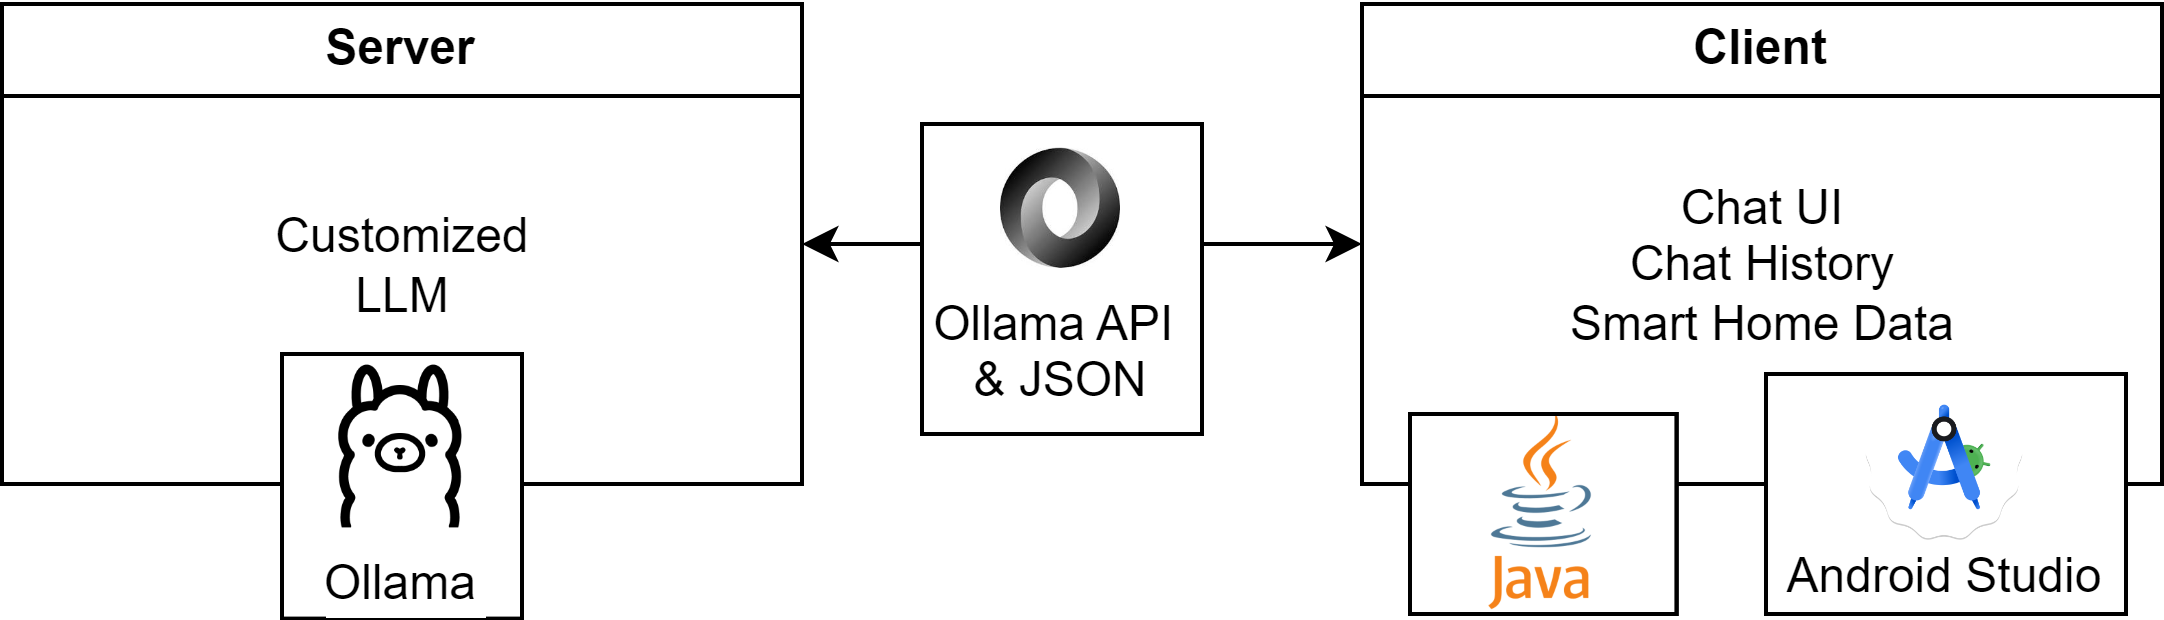
\includegraphics[width=0.9\textwidth]{graphics/techstack.png}
    \caption{Technology Stack Visualized on Base Architecture}
    \label{fig:techstack}
\end{figure}

\section{Server}
This section covers the server-side implementation of the Smart Home Chatbot system. 
It details the initial plan to use bwCloud and the challenges that led to switching to a private computer setup. 
We discuss the hardware specifications of the server and how it affects model performance and response times. 
The section also explains the deployment of Ollama for hosting and customizing language models. 
We then dive into the process of model selection, considering factors like parameter count, popularity, and language support. 
Finally, we explore the techniques used for model customization, including the creation of modelfiles and prompt engineering, to tailor the language models for smart home interactions.

\subsection{Hardware and Performance}
\label{subsec:hardware}
The initial plan was to use the bwCloud\footnote{\url{https://www.bw-cloud.org/}}, a currently free service that can be used of students and researchers of different institutions accross Baden-Württemberg, Germany.
It was easy to get the needed resources for this project which where eigth VCPUs, 16GB RAM and also enough memory for the size of the \glspl{llm} that were planned to use.
When trying out to run models directly on the server the response times were okay for models up to approximately 10 Billion parameters although the used server has no GPU.
However, when testing customized models through HTTP Requests the response times were much higher than expected.
Especially the first response often took over one minute with preceeding requests taking minimum 30 seconds depending on the length of the generated respone.
The first request usually takes longer when the model used is not already loaded into the RAM.

Because of the occuring difficulties and with wanting to use as low budget as possible we decided to use an existing private Computer with more Resources and used IPv6 Host Exposure for a specific port on which the Ollama \gls{api} was running.
The computer had an NVIDIA GeForce 980 ti graphics card with 6GB VRAM and 32GB RAM with 3600MHz.
Even longer model responses usually only took a few seconds to receive.

\subsection{Model Customization}
\label{subsec:modelcust}
This section is all about the language models themselves. It covers which model where selected and why, how the models where customized with so called ``Modelfiles'' and an engineered prompt.
\subsubsection{Model Selection}
Initially the model in the focus of this work was llama3 since it was one of the most recent models and seen everywhere when starting with the thesis.
However, it makes sense to try out other models and see how they perform therefore we came up with a solid model selection which can be seen in \cref{tab:models-used}.
The model selection was based on parameter count, popularity, ranking in the \gls{bfcl} and availability in the ollama models library.
Another condition for the model was to support German.
The parameter count should be lower than 15 Billion since it wouldn't really run on the server setup described in the last section.
The model should be either under the most popular models filter on the Ollama library website \footnote{\url{https://ollama.com/library?sort=popular}}

% Define a new column type 'Y' for wider last column
\newcolumntype{Y}{>{\hsize=1.2\hsize}X}
\begin{table}[h!]
    \centering
    \begin{tabularx}{\textwidth}{lXXp{3cm}Xl}
    \toprule
    Model & Parameters & Size & Popularity \newline (Ollama) & BFCL \newline Accuracy & Organization \\
    \midrule
    home-3b-v3 & 3b & 1.7GB & 2.3K & - & - \\
    qwen2-7b-instruct & 7b & 4.4GB & 281.6K & - & Alibaba \\
    qwen2-1.5b-instruct & 1.5b & 0.9GB & 281.6K & - & Alibaba \\
    mistral-7b-instruct & 7b & 4.1GB & 2.8M & - & Mistral AI \\
    gemma-2b-instruct & 2b & 1.7GB & 3.9M & - & Google \\
    gemma-instruct & 7b & 5GB & 3.9M & 43.82 & Google \\
    zephyr & 7b & 4.1GB & 107.8K & - & Mistral AI \\
    llama3 & 8b & 4.7GB & 4.5M & - & Meta \\
    llama3-instruct & 8b & 4.7GB & 4.5M & 60.29 & Meta \\
    phi2 & 2.7b & 1.6GB & 200.1K & - & Microsoft \\
    phi3-3.8b & 3.8b & 2.2GB & 2.1M & - & Microsoft \\
    phi3-14b & 14b & 7.9GB & 2.1M & - & Microsoft \\
    gemma2 & 9b & 5.4GB & 290.1K & - & Google \\
    gorilla-openfunctions-v2 & 6.9b & 2.7GB & <1K & 84.65 & Gorilla LLM \\
    \bottomrule
    \end{tabularx}
    \caption{Overview of the Models Used}
    \label{tab:models-used}
\end{table}

Here are some additional notes to this table:
\begin{itemize}
    \item The model \textit{home-3b-v3} was selected because it was fine-tuned to control devices with Home Assistant \cite{acon96_home_llm}.
    \item Only the commercial models from \textit{Mistral AI} are on the BCFL.
    \item \textit{Gemma2} and \textit{Phi3} were released later in the thesis phase, so \textit{gemma} and \textit{phi2} were also used.
    \item We noticed that the \textit{instruct} version of \textit{llama3} performed slightly better for our task than the plain version. Therefore, we usually preferred the instruct versions of other models if available.
    \item The model \textit{gorilla-openfunctions-v2} was not added to Ollama by Gorilla LLM but by a user who made it executable on Ollama.
    \item The \gls{bfcl} accuracy rating is according to the following date: 2024-07-06
    \item The popularity in the Ollama library is based on the amount of pulls of a model. It is one count per model which includes each different version of the model (e.g. instruct, different sizes).
\end{itemize}


\subsubsection{Modelfiles}
Modelfiles are configuration files used to customize and fine-tune language models for specific applications. They allow developers to define instructions, examples, and parameters that guide the model's behavior, ensuring more accurate and contextually appropriate responses. In the context of this project, modelfiles were crucial for tailoring the language model to understand and interact with the Bosch Smart Home system effectively.
The Ollama software uses modelfiles to create and share models. Let's examine the key components of our custom modelfile for the Bosch Smart Home chatbot:

\begin{Listing}[b]
\begin{lstlisting}[language=bash]
FROM llama3:instruct
PARAMETER temperature 0.95
\end{lstlisting}
\caption{Base Model and Temperature Setting}
\label{lst:base_model}
\end{Listing}

The section in \cref{lst:base_model} specifies the base model (llama3:instruct) and sets the temperature parameter. As shown in this listing, the temperature value of 0.95 allows for more creative responses while maintaining coherence.

\begin{Listing}
\begin{lstlisting}[language=bash]
SYSTEM """
You are 'SHBot' (Smart Home Bot), a helpful AI Assistant that controls smart home devices. Complete tasks or answer questions based on a provided device list. Always respond in the language of the user request and keep answers brief.
Answer in the following format containing a natural language response to the user and a json:
natural language answer to the user
{
'action': 'intent/action',
'value': 'optional value for an action',
'deviceID': 'ID of the device',
'device': 'device type',
'room': 'device room',
'name': 'device name'
}
Important: Always place the json at the end of your response.
"""
\end{lstlisting}
\caption{System Message - Part 1: Role Definition and Response Format}
\label{lst:system_message_1}
\end{Listing}

Listing \ref{lst:system_message_1} shows the first part of the system message, which defines the bot's role and sets the expected response format. It instructs the model to provide both a natural language answer and a structured \gls{json} output, which is crucial for integrating the chatbot's responses with the smart home system.

\begin{Listing}
\begin{lstlisting}[language=bash]
SYSTEM """
Available Actions:
'none', 'turn-on', 'turn-off', 'change-temperature(value needed)'
Devices:
'socket': can use 'turn-on' and 'turn-off'
'thermostat' or 'RADIATOR_THERMOSTAT': The measured temperature can be viewed on each individual thermostat (RADIATOR_THERMOSTAT). It is typically structured like this: "id": "TemperatureLevel", "state": { "temperature": 22.5 }
'room-climate-control': can use 'change-temperature(value)'. This is a virtual device in the smart home that manages the temperature (called setPointTemperature) of the thermostats in the same room. If no thermostat exists, the system won't create a room climate control.
'door-window-contact': can't use the actions, only provides information whether its opened or closed.
"""
\end{lstlisting}
\caption{System Message - Part 2: Available Actions and Device Types}
\label{lst:system_message_2}
\end{Listing}

Listing \ref{lst:system_message_2} outlines the available actions and device types in the Bosch Smart Home system. This section provides the model with crucial information about the capabilities and limitations of each device type, enabling more accurate responses to user queries.

\begin{Listing}
\begin{lstlisting}[language=bash]
SYSTEM """
Example conversations:
For this example assume the user has the following devices:
'[{"type": "POWER_METER_SWITCH", "name": "TV", "deviceID": "device123", "state": [{"id": "PowerSwitch", "state": {"switchState": "OFF"}}], "room": "Schlafzimmer"}, {"type": "SHUTTER_CONTACT", "name": "WindowSensor-67890", "deviceID": "device456", "state": [{"id": "ShutterContact", "state": {"value": "CLOSED"}}], "room": "Wohnzimmer"}]'

MESSAGE user Can you turn on my TV?
MESSAGE assistant Sure, turning on the TV now. { "action": "turn-on", "deviceID": "device123", "device": "POWER_METER_SWITCH", "room": "Schlafzimmer", "name": "TV" }
"""
\end{lstlisting}
\caption{Example Conversations and Device List}
\label{lst:example_conversations}
\end{Listing}

\paragraph{Using Example User Inputs for the Modelfiles} 
Listing \ref{lst:example_conversations} provides example conversations to guide the model's responses. It includes a sample device list and demonstrates how the model should interpret user queries and format its responses, including the use of different languages and the structured \gls{json} output.
A significant aspect of our model customization process involved leveraging the example user inputs collected during our survey mentioned in \cref{sec:collectinputs}. We carefully selected a subset of these inputs to include in the modelfile used for customizing the selected \glspl{llm}. This approach allowed us to fine-tune the models with real-world, domain-specific examples, enhancing their ability to understand and respond to typical smart home queries. By incorporating these authentic user inputs into the model's training data, we aimed to improve its contextual understanding and response accuracy for smart home-related interactions and therefore create a more domain-specfic model.

By incorporating these detailed instructions and examples, as shown in Listings \ref{lst:base_model} through \ref{lst:example_conversations}, the modelfile ensures that the language model can effectively understand and respond to user queries about their Bosch Smart Home devices, providing accurate information and executing commands as needed.


\subsubsection{Prompt Engineering}

Prompt engineering is the process of designing and refining input prompts to elicit desired responses from language models. It involves crafting specific instructions, context, and examples to guide the model's output effectively. In the context of our Bosch Smart Home chatbot, prompt engineering was crucial for ensuring accurate and relevant responses to user queries about their smart home devices.

The process of building the prompt is closely intertwined with the development of the modelfile. In our modelfile, we defined how the model should act and specified that it would be provided with a device list for each user. This integration of prompt engineering and modelfile development was essential for creating a cohesive and effective chatbot system.

For our Bosch Smart Home chatbot, we implemented a message history approach for prompt engineering. This method involves including the user's device list as the first message in the conversation history, followed by the user's actual query. This approach proved to be intuitive, straightforward to implement on the client side, and allowed us to maintain flexibility in model selection while providing necessary context for accurate responses.
For a more detailed discussion of the prompt engineering process, including alternative approaches considered, please refer to \cref{sec:prompteng-appendix}.

\section{Client}
This section provides details about all the components at the client-side as approached in \cref{sec:design}. 
The client-side implementation is a crucial part of the Smart Home Chatbot system, handling user interactions, data management, and communication with the server. It extends the existing Bosch Smart Home Android app, integrating new functionalities while maintaining consistency with the app's design and user experience. 
The following subsections break down the various aspects of the client implementation, including how data is managed, the user interface design, message handling, request construction, and response processing. 

\subsection{Data Management}
Additionally to the \gls{json} data exchange between client and server the data of the smart home itself has to be managed in order to put it into the \gls{json} and transmit it and also handle the \gls{json} received from the server.
The Bosch Smart Home app has an internal data model to store the current state of the users smart home. It updates this model when starting the app and on certain events.
Therefore, two options were available for managing the device data: either using the available data model or sending requests through the available internal \gls{api} of the system.
To keep the latency low we decided to use the internal data model and filter relevant data out. As described in \cref{subsec:devices} three devices were considered for the prototype.
Therefore we only used data relevant for the user from this devices. Since there was much unnecessary data in each device state we collected only the data described in \cref{tab:device_state_data_detailed}.
Of course when controlling devices the data model has to be updated in parallel to updating the devices themselves.
\begin{table}[h!]
    \centering
    \begin{tabularx}{\textwidth}{|p{3cm}|X|}
    \hline
    \textbf{Device Type} & \textbf{Collected State Data} \\ \hline
    Smart Plug & 
    \textbf{powerConsumption}: Current power usage in watts \newline
    \textbf{energyConsumption}: Total energy consumed over time in kilowatt-hours \newline
    \textbf{switchState}: Whether the device is turned ON or OFF \\ \hline
    Thermostat & 
    \textbf{valvePosition}: Position of the radiator valve \newline
    \textbf{childLock}: Whether the child lock is ON or OFF \newline
    \textbf{temperature}: Current temperature measured by the thermostat in Celsius \\ \hline
    Room Climate Control & 
    This is not a real device. It is virtually managing all thermostats in one room to achieve a desired temperature.
    \textbf{ventilationMode}: Whether ventilation mode is active. \newline
    \textbf{boostMode}: Whether boost mode is active. This mode is used to increase the heat output for a short time \newline
    \textbf{operationMode}: Current operation mode (automatic or manual) \newline
    \textbf{setpointTemperature}: Desired temperature set by the user in Celsius \newline
    \textbf{currentTemperature}: Actual room temperature in Celsius \\ \hline
    Door Window Contact & 
    \textbf{contactState}: Whether the window or door is OPEN or CLOSED \\ \hline
    \end{tabularx}
    \caption{Detailed State Data Collected from Different Smart Home Devices}
    \label{tab:device_state_data_detailed}
\end{table}

Another point for data management are the system logs of the Bosch Smart Home system (and potentially additional historical data) to for example reason why something happened in the system and data from external sources to for example analyze how the electricity price changed.
Since we were not able to implement this it is mentioned in \cref{sec:challenges-solutions}.


\subsection{User Interface}
\label{sec:ui}
% in the main activity in the Bosch Smart Home app multiple views can be selected in the bottom like "Favourites" and "Room". The Toolbar in the top is always shown while in the main activity. Extending this existing functionality we added a button saying "CHATBOT" to the toolbar which can be seen in \cref{fig:ui-homescreen} to have the chatbot functionality available no matter where you are currently in the main activity. This provides a simple but efficient way to get to the chatbot.
% In \cref{fig:chatactivity} an overview of the actual chatbot \gls{ui} is shown. The toolbar here consists of an "Up Button" how it is often called in Android which is just a button to get back to the main activity. It also has an heading "Smart Home Chatbot".
% Directly under the toolbar another bar is shown which is more of an development feature. It makes it possible to select different models (that can also correspond to different endpoints) through a dropdown (spinner) and is shown more detailed in \cref{fig:model-select}. A message is always sent to the currently selected model/endpoint.
% Just below this model selection the heart of the chatbot \gls{ui} can be seen which is the chat history consisting of the messages the user wrote at the right in an olive green and the messages of ``SHBot'' (abbreviation of Smart Home Chatbot) on the left with white background. The time on which a message was sent/received is also shown.
% The message history shown in \cref{fig:ui-chatactivity} shows a conversation about the functionality of the chatbot. As you can see it summarized its functionality quite well by describing possible action, providing an example and also limitations. Only a bit buggy is the last sentence which is probably due to the fact that the chatbot usually answers with natural language in the beginning and a \gls{json} in the end of a message.
% As a note: the chat history is only persisted in the current session and is lost upon reentering the chatbot activity which was sufficient for the prototypical use.
% In the bottom of the whole chatbot \gls{ui} the input field for the user and a button to send his message are available. When clicking on the field the keyboard of the Android device expands.
% In our case the keyboard also has feature to use speech-to-text.
\begin{figure}[!b]
    \centering
      \begin{subfigure}[t]{.44\textwidth}
        \vspace*{0pt}
        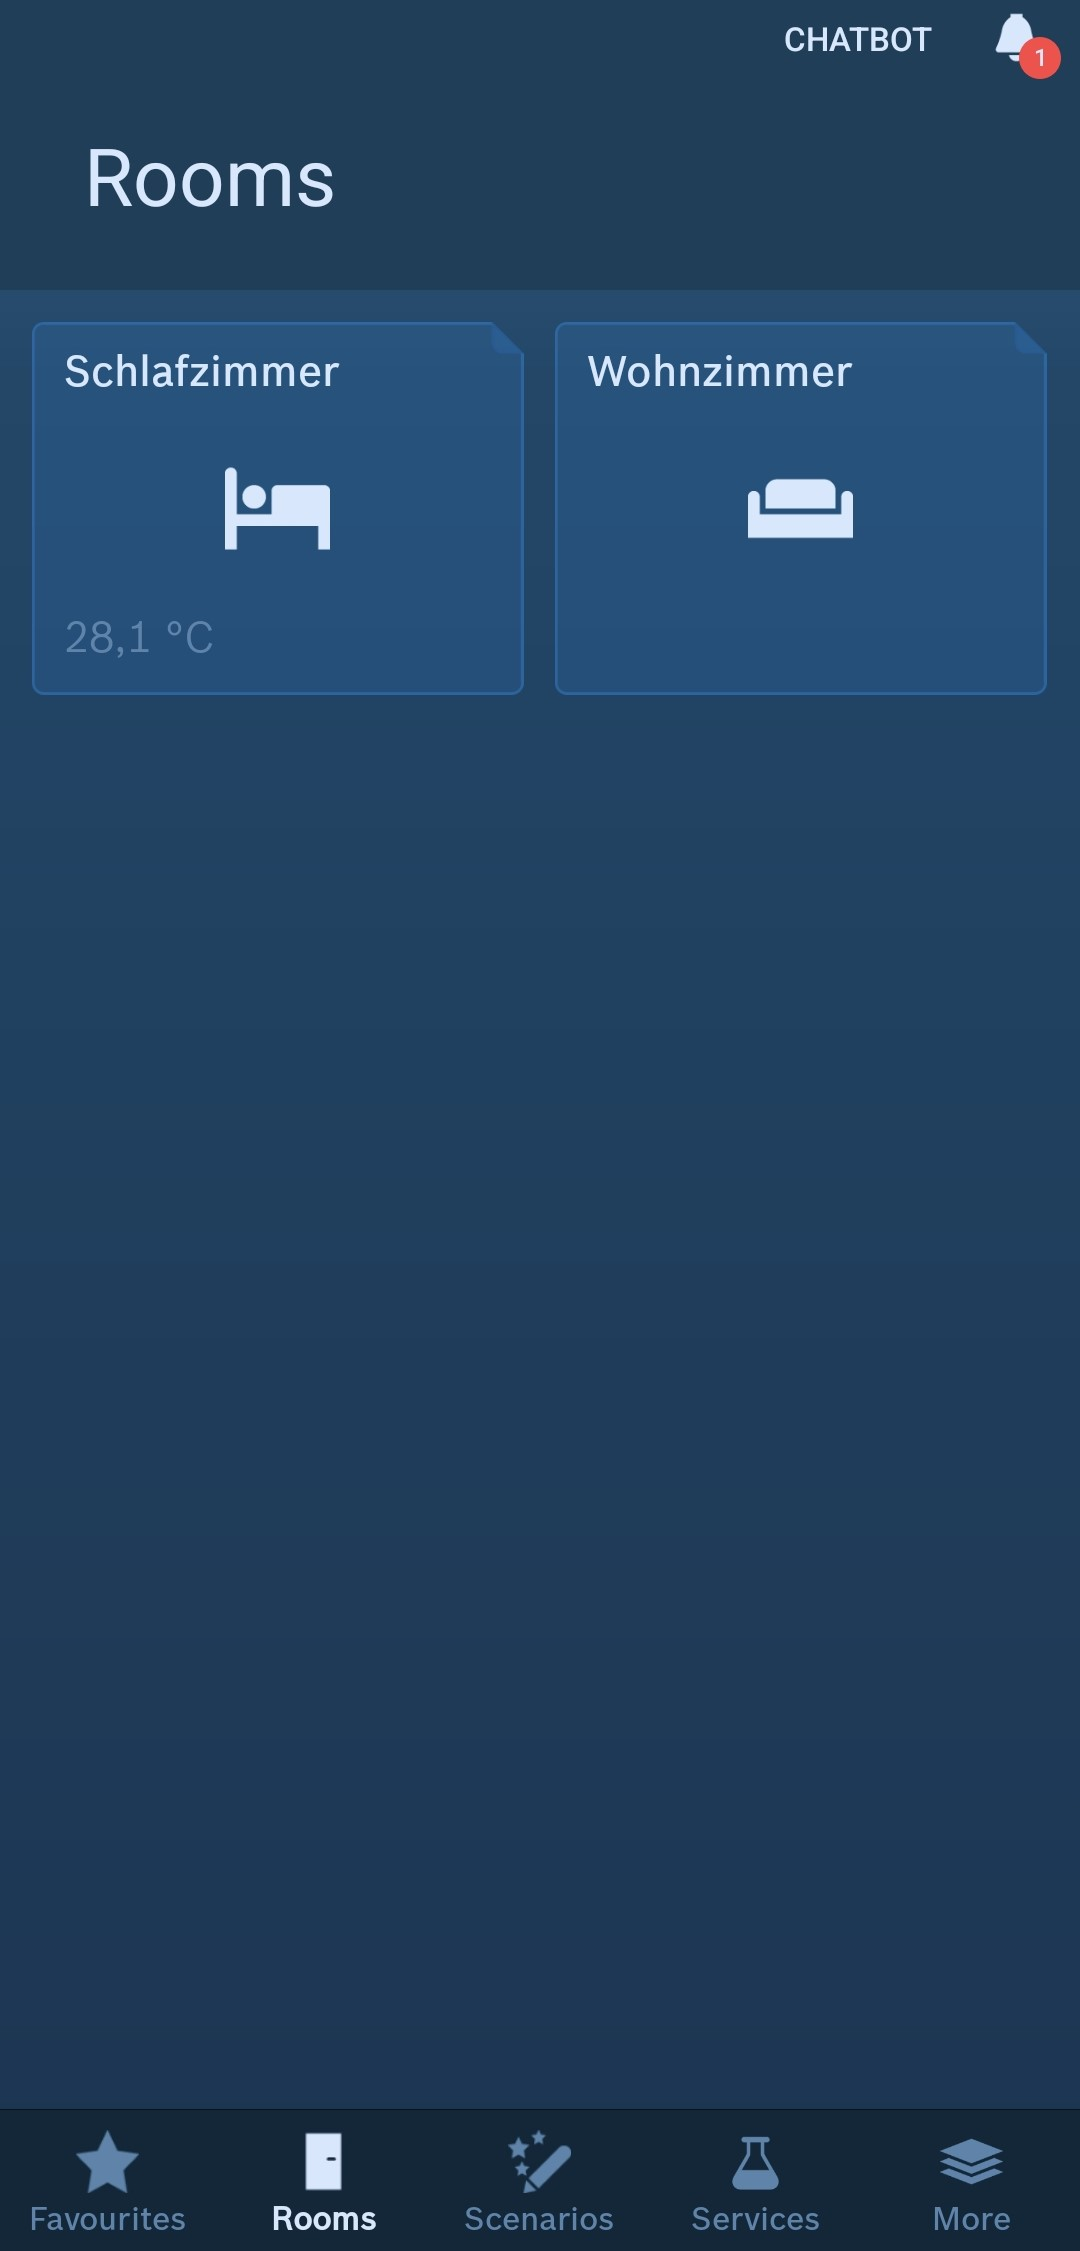
\includegraphics[width=\textwidth]{graphics/homescreen.jpg}
        \caption{Availability of the chatbot in the main app activity}
        \label{fig:ui-homescreen}
      \end{subfigure} \hfill
      \begin{subfigure}[t]{.44\textwidth}
        \vspace*{0pt}
        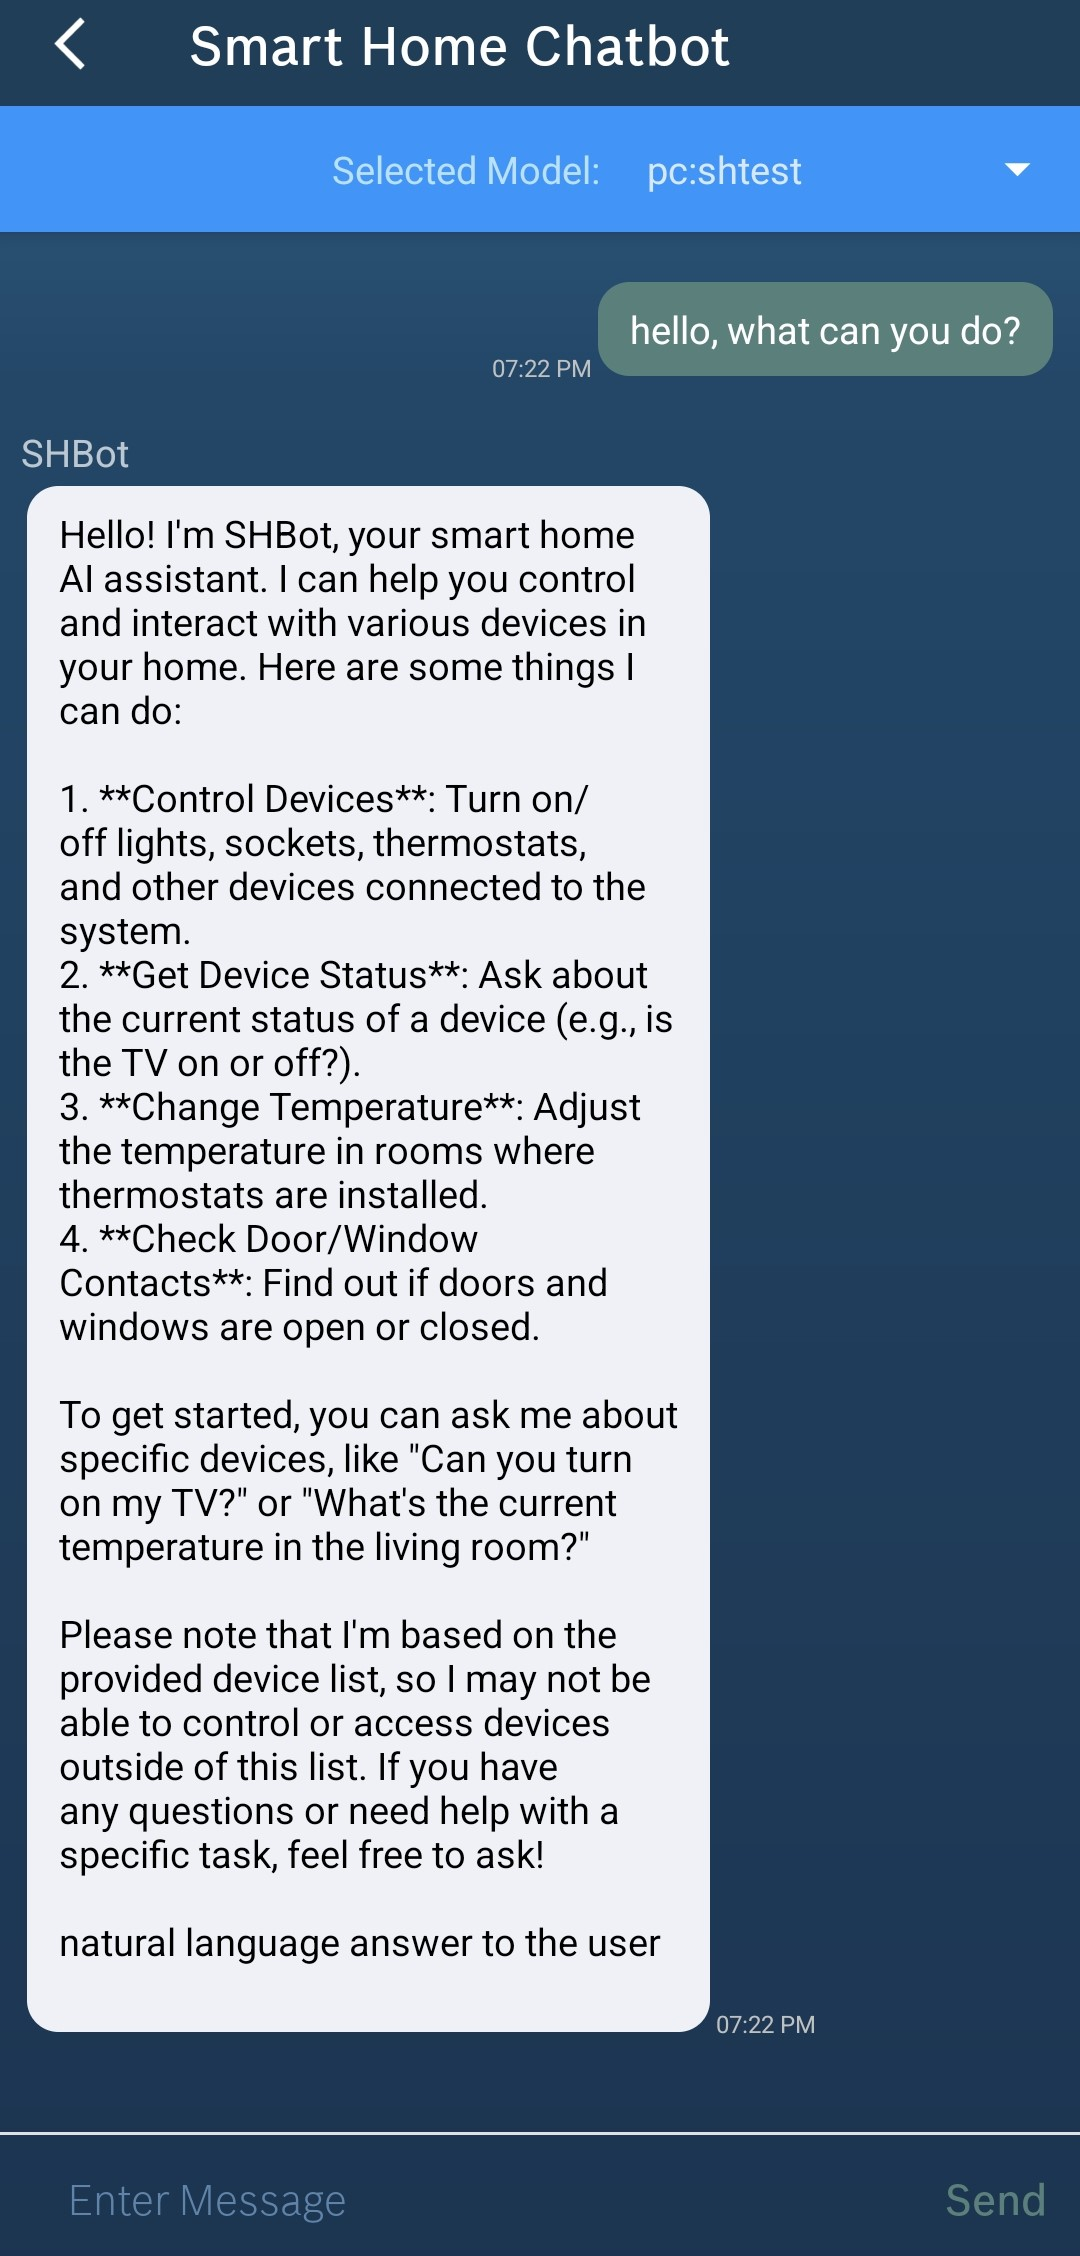
\includegraphics[width=\textwidth]{graphics/chatactivity.jpg}
        \caption{View of the chatbot activity}
        \label{fig:ui-chatactivity}
        \end{subfigure}
      \caption{Overview of the User Interface}
      \label{fig:ui-overview}
\end{figure}
The user interface of our Smart Home Chatbot was designed to seamlessly integrate with the existing Bosch Smart Home app while providing easy access to the chatbot functionality. Figure \ref{fig:ui-overview} provides an overview of the user interface implementation.
The chatbot activity is built upon the Android AppCompatActivity class, ensuring compatibility across different Android versions and providing a consistent look and feel with the rest of the application.
In the main activity of the Bosch Smart Home app, users can select multiple views such as ``Favourites'' and ``Rooms'' using the bottom navigation. To make the chatbot easily accessible from any part of the main activity, we extended the existing functionality by adding a ``CHATBOT'' button to the toolbar, as shown in Figure \ref{fig:ui-homescreen}. This simple yet efficient solution allows users to access the chatbot from anywhere within the main activity.

Figure \ref{fig:ui-chatactivity} displays the layout of the chatbot \gls{ui}. The toolbar features an ``Up Button'', a common Android navigation element, allowing users to return to the main activity. The toolbar also includes the heading  ``Smart Home Chatbot'' for clear identification.
Below the toolbar, we implemented a development feature that allows selection of different models or endpoints through a dropdown menu (spinner), as detailed in Figure \ref{fig:model-select}. This feature enables testing and comparison of various models during development. Messages are always sent to the currently selected model/endpoint.

The core of the chatbot \gls{ui} is the chat history, displayed below the model selection. User messages appear on the right side in olive green, while responses from ``SHBot'' (Smart Home Chatbot) are shown on the left with a white background. Each message includes a timestamp indicating when it was sent or received.
A notable feature of the chatbot's response mechanism is the real-time display of each token as it is received from the language model. This creates the effect of the chatbot ``writing'' its response in real-time, enhancing the interactive feel of the conversation and providing immediate feedback to the user.
The conversation shown in Figure \ref{fig:ui-chatactivity} demonstrates the chatbot's ability to summarize its functionality, describing possible actions, providing examples, and outlining limitations. A minor inconsistency is noted in the last sentence, likely due to the chatbot's typical response format of natural language followed by \gls{json} data. For more example conversations see \cref{sec:chatbot-conv}.
It's worth noting that the chat history is only maintained for the current session and is not persisted when re-entering the chatbot activity, which was deemed sufficient for the prototype.

\begin{figure}[!tbh]
    \centering
      \begin{subfigure}[t]{.48\textwidth}
        \vspace*{0pt}
        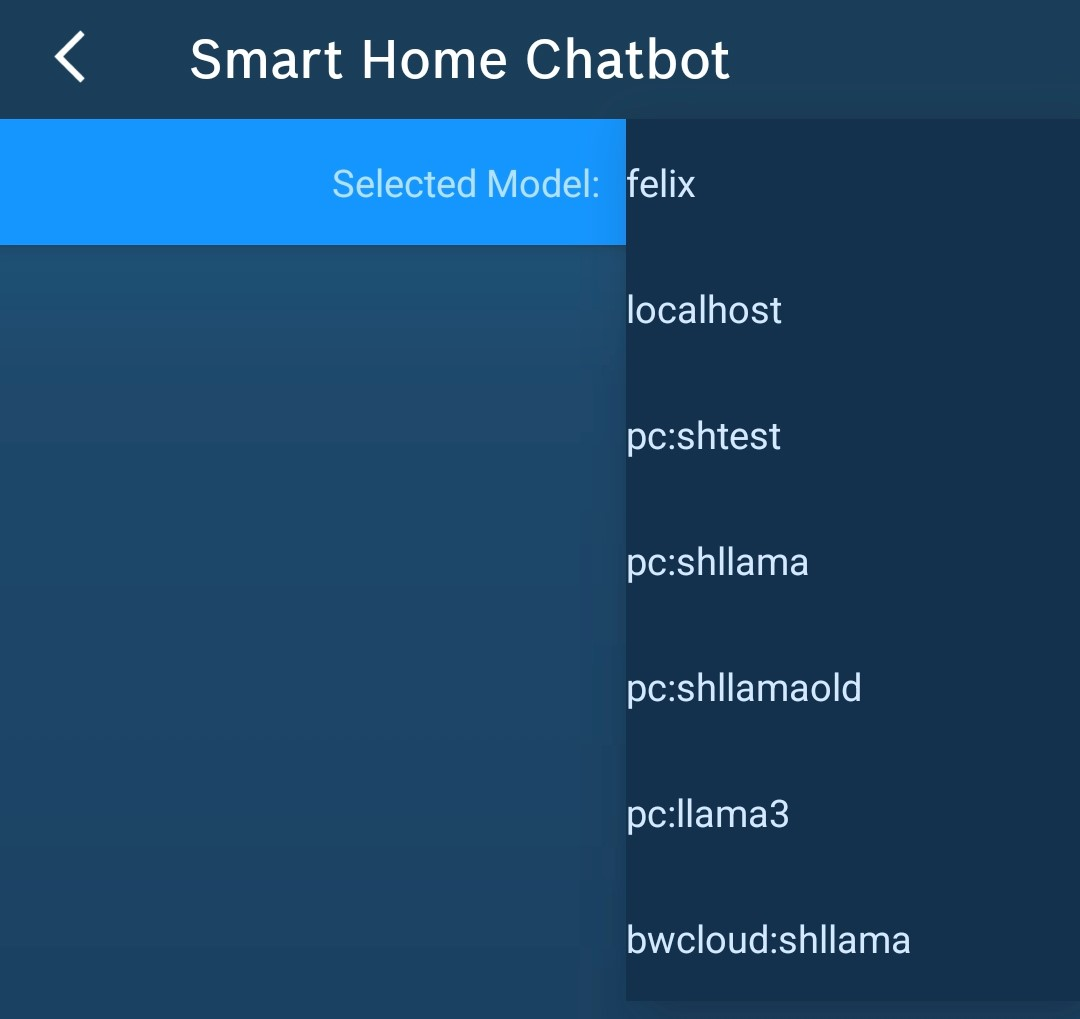
\includegraphics[width=\textwidth]{graphics/model-select.jpg}
        \caption{Expanded Model Selection}
        \label{fig:model-select}
      \end{subfigure} \hfill
      \begin{subfigure}[t]{.43\textwidth}
        \vspace*{0pt}
        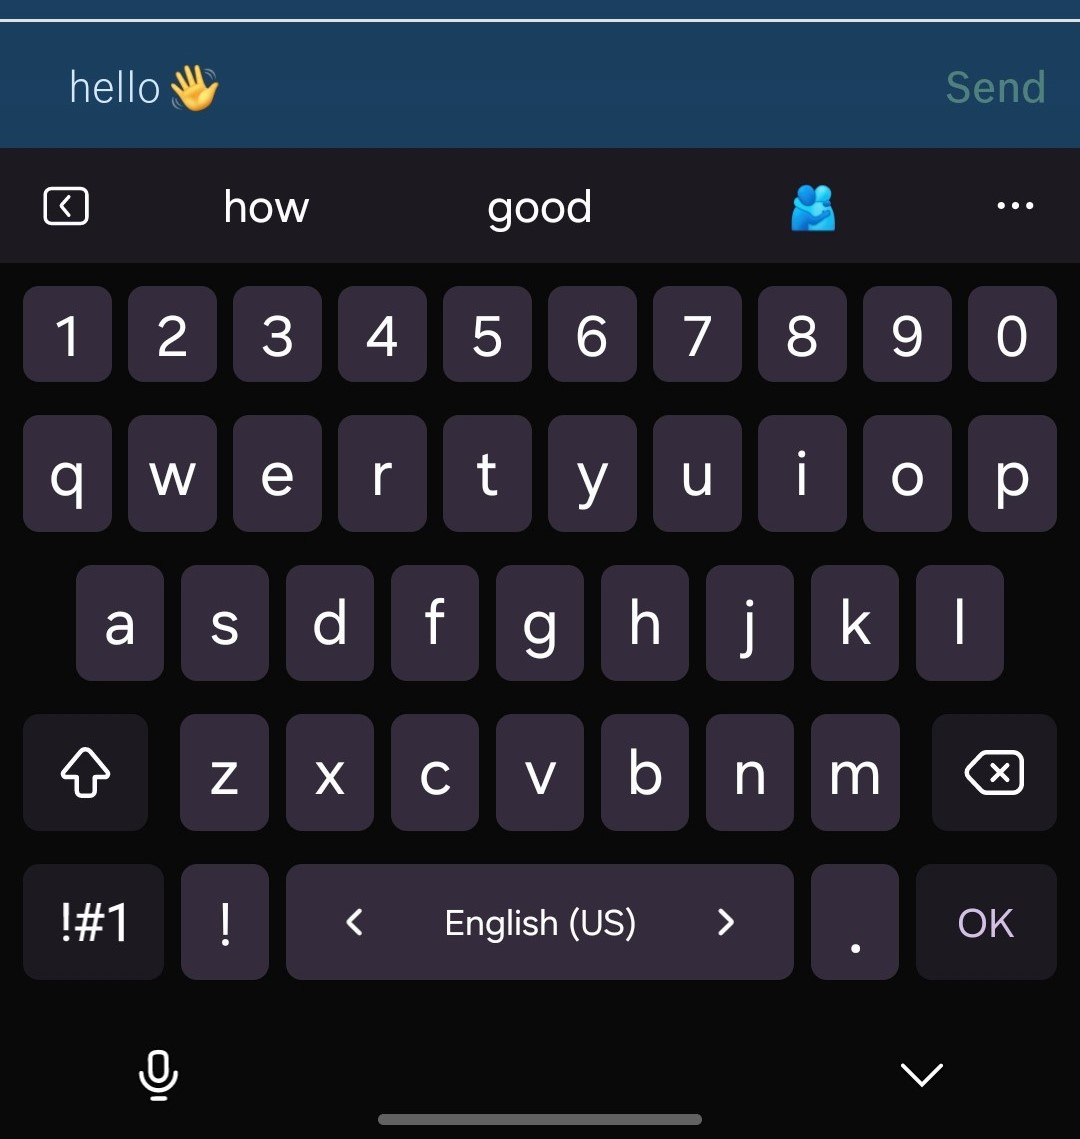
\includegraphics[width=\textwidth]{graphics/keyboard.jpg}
        \caption{View when writing a message}
        \label{fig:keyboard}
        \end{subfigure}
      \caption{Details of the Chatbot User Interface}
      \label{fig:ui-details}
\end{figure}

At the bottom of the chatbot \gls{ui}, users can find an input field for typing messages and a send button. When the input field is selected, the Android device's keyboard appears, as shown in Figure \ref{fig:keyboard}. The keyboard also includes a speech-to-text feature, enhancing accessibility and user convenience.
Figure \ref{fig:ui-details} provides additional details of the chatbot user interface, showcasing the expanded model selection dropdown and the view when composing a message.

This user interface design, built on AppCompatActivity, ensures that the Smart Home Chatbot is easily accessible, intuitive to use, and seamlessly integrated with the existing Bosch Smart Home app functionality. The real-time token display feature adds a dynamic and engaging element to the user experience.

\subsection{Request Building}
\label{sec:req-building}
As previously described in \cref{subsec:apiclient}, the Request Builder within the \gls{api} Client \& Request Builder module constructs properly formatted \gls{api} requests, sends them, parses server responses, and handles asynchronous operations.
This section elaborates on the process of building and sending these requests.

\captionsetup[lstlisting]{labelformat=empty}
\begin{Listing}[h]
\begin{minipage}{0.53\textwidth}
    \begin{lstlisting}[caption={Base Structure of each POST Request}, label=lst:first, frame=single]
POST http://<domain-placeholder>/api/chat
{
    "model": "<model-placeholder>",
    "messages": [
    {
        "role": "user",
        "content": "<device-list-placeholder>"
    },
    {
        "role": "user",
        "content": "<user-message-placeholder>"
    }
    ],
    "stream": true
}
    \end{lstlisting}
    \end{minipage}
    \hfill
    \begin{minipage}{0.4\textwidth}
    \vspace{10pt}
    \begin{lstlisting}[caption={Example Device List containing only a Smart Plug}, label=lst:second, frame=single]
[{
    "type": "POWER_METER_SWITCH",
    "name": "Office Desk Lamp",
    "deviceID": "12345",
    "state": [
        {
        "id": "PowerMeter",
        "state": {
            "powerConsumption": 10,
            "energyConsumption": 50
        }
        },
        {
        "id": "PowerSwitch",
        "state": {
            "switchState": "ON"
        }
        }
    ],
    "room": "Office"
}]
    \end{lstlisting}
    \end{minipage}
    \caption{Components of a POST Request to the Server Running Ollama}
    \label{lst:post-request}
\end{Listing}
\captionsetup{labelformat=default}

To ensure low latency while maintaining context, the system considers only a limited number of recent messages when constructing a request. Importantly, the first message in the history always contains a list of the user's devices, providing crucial context for the language model.
The message history follows a strict alternating pattern between ``user'' and ``assistant'' roles after the initial device list. When a user sends a new message, it is appended to this structured history, ensuring the language model has sufficient context for accurate reasoning.
\cref{lst:post-request} illustrates the format of a POST request sent to the server. The 'messages' array encapsulates the condensed message history, with the user's latest message positioned at the end. This structure provides the language model with a concise yet comprehensive context for generating appropriate responses.

The 'model' field specifies the language model to be used, while the 'stream' parameter set to true enables real-time streaming of the model's response. This approach allows for immediate display of partial responses, enhancing the user experience by reducing perceived latency.
The device list, exemplified in the right panel of \cref{lst:post-request}, provides detailed information about each smart home device, including its type, name, unique identifier, current state, and location. This comprehensive device context enables the language model to generate informed and relevant responses to user queries about their smart home environment.


\subsection{Response Handling and Action Triggering}
As previously described in \cref{subsec:responsehandler}, the Response Handler module interprets server responses, determining necessary client actions such as response analysis and orchestration. The response handling is closely integrated with the \gls{api} Client, which parses the server responses and initiates the response handling process. This section elaborates on the implementation details of this crucial functionality.
The response from the server, as initiated by the request detailed in \cref{sec:req-building}, is received as a stream of tokens through the Ollama software. This streaming approach allows for real-time processing and display of the model's output, enhancing the responsiveness of the chatbot interface.
While receiving the response stream, the handler separates it into two components:

\textbf{Natural Language Response: This portion} is immediately forwarded to the \gls{ui} for display, maintaining a fluid conversation flow with the user.\\
\textbf{\gls{json} Object:} Typically positioned at the end of the response, this structured data undergoes parsing to extract action-related information.

The \gls{json} object, as defined in the modelfile (see \cref{lst:system_message_1}), contains key information for action triggering (only listed the important ones here):

\begin{itemize}
\item 'action': Specifies the intent or action to be performed
\item 'value': An optional parameter for actions requiring additional data
\item 'deviceID': Unique identifier of the target device
\end{itemize}

The Response Handler processes this \gls{json} object to determine the appropriate action. As outlined in \cref{lst:system_message_2}, the system supports several actions:

\begin{itemize}
\item 'none': No action required
\item 'turn-on': Activate a device (e.g., a smart socket)
\item 'turn-off': Deactivate a device
\item 'change-temperature': Adjust temperature settings (requires a 'value' parameter)
\end{itemize}

Based on the 'action', 'deviceID' and eventually the 'value' fields in the \gls{json}, the Response Handler triggers the corresponding function in the client application with correct prarameters. For instance:

\begin{itemize}
\item If the action is 'turn-on' or 'turn-off', it calls the appropriate method to change the state of the specified device (identified by 'deviceID').
\item For 'change-temperature', it invokes the temperature adjustment function for the room climate control device, using the provided 'value'.
\item In case of 'none', no further action is taken beyond displaying the natural language response.
\end{itemize}

The main challenge here was to design a robust parsing mechanism for mapping the received \gls{json} to the exact functionality wanted.
The Response Handler also manages error scenarios, such as invalid actions or device IDs not present in the current device list.


\section{Interaction Flow}
\begin{figure}[!bht]
    \centering
    \captionsetup{justification=centering}
    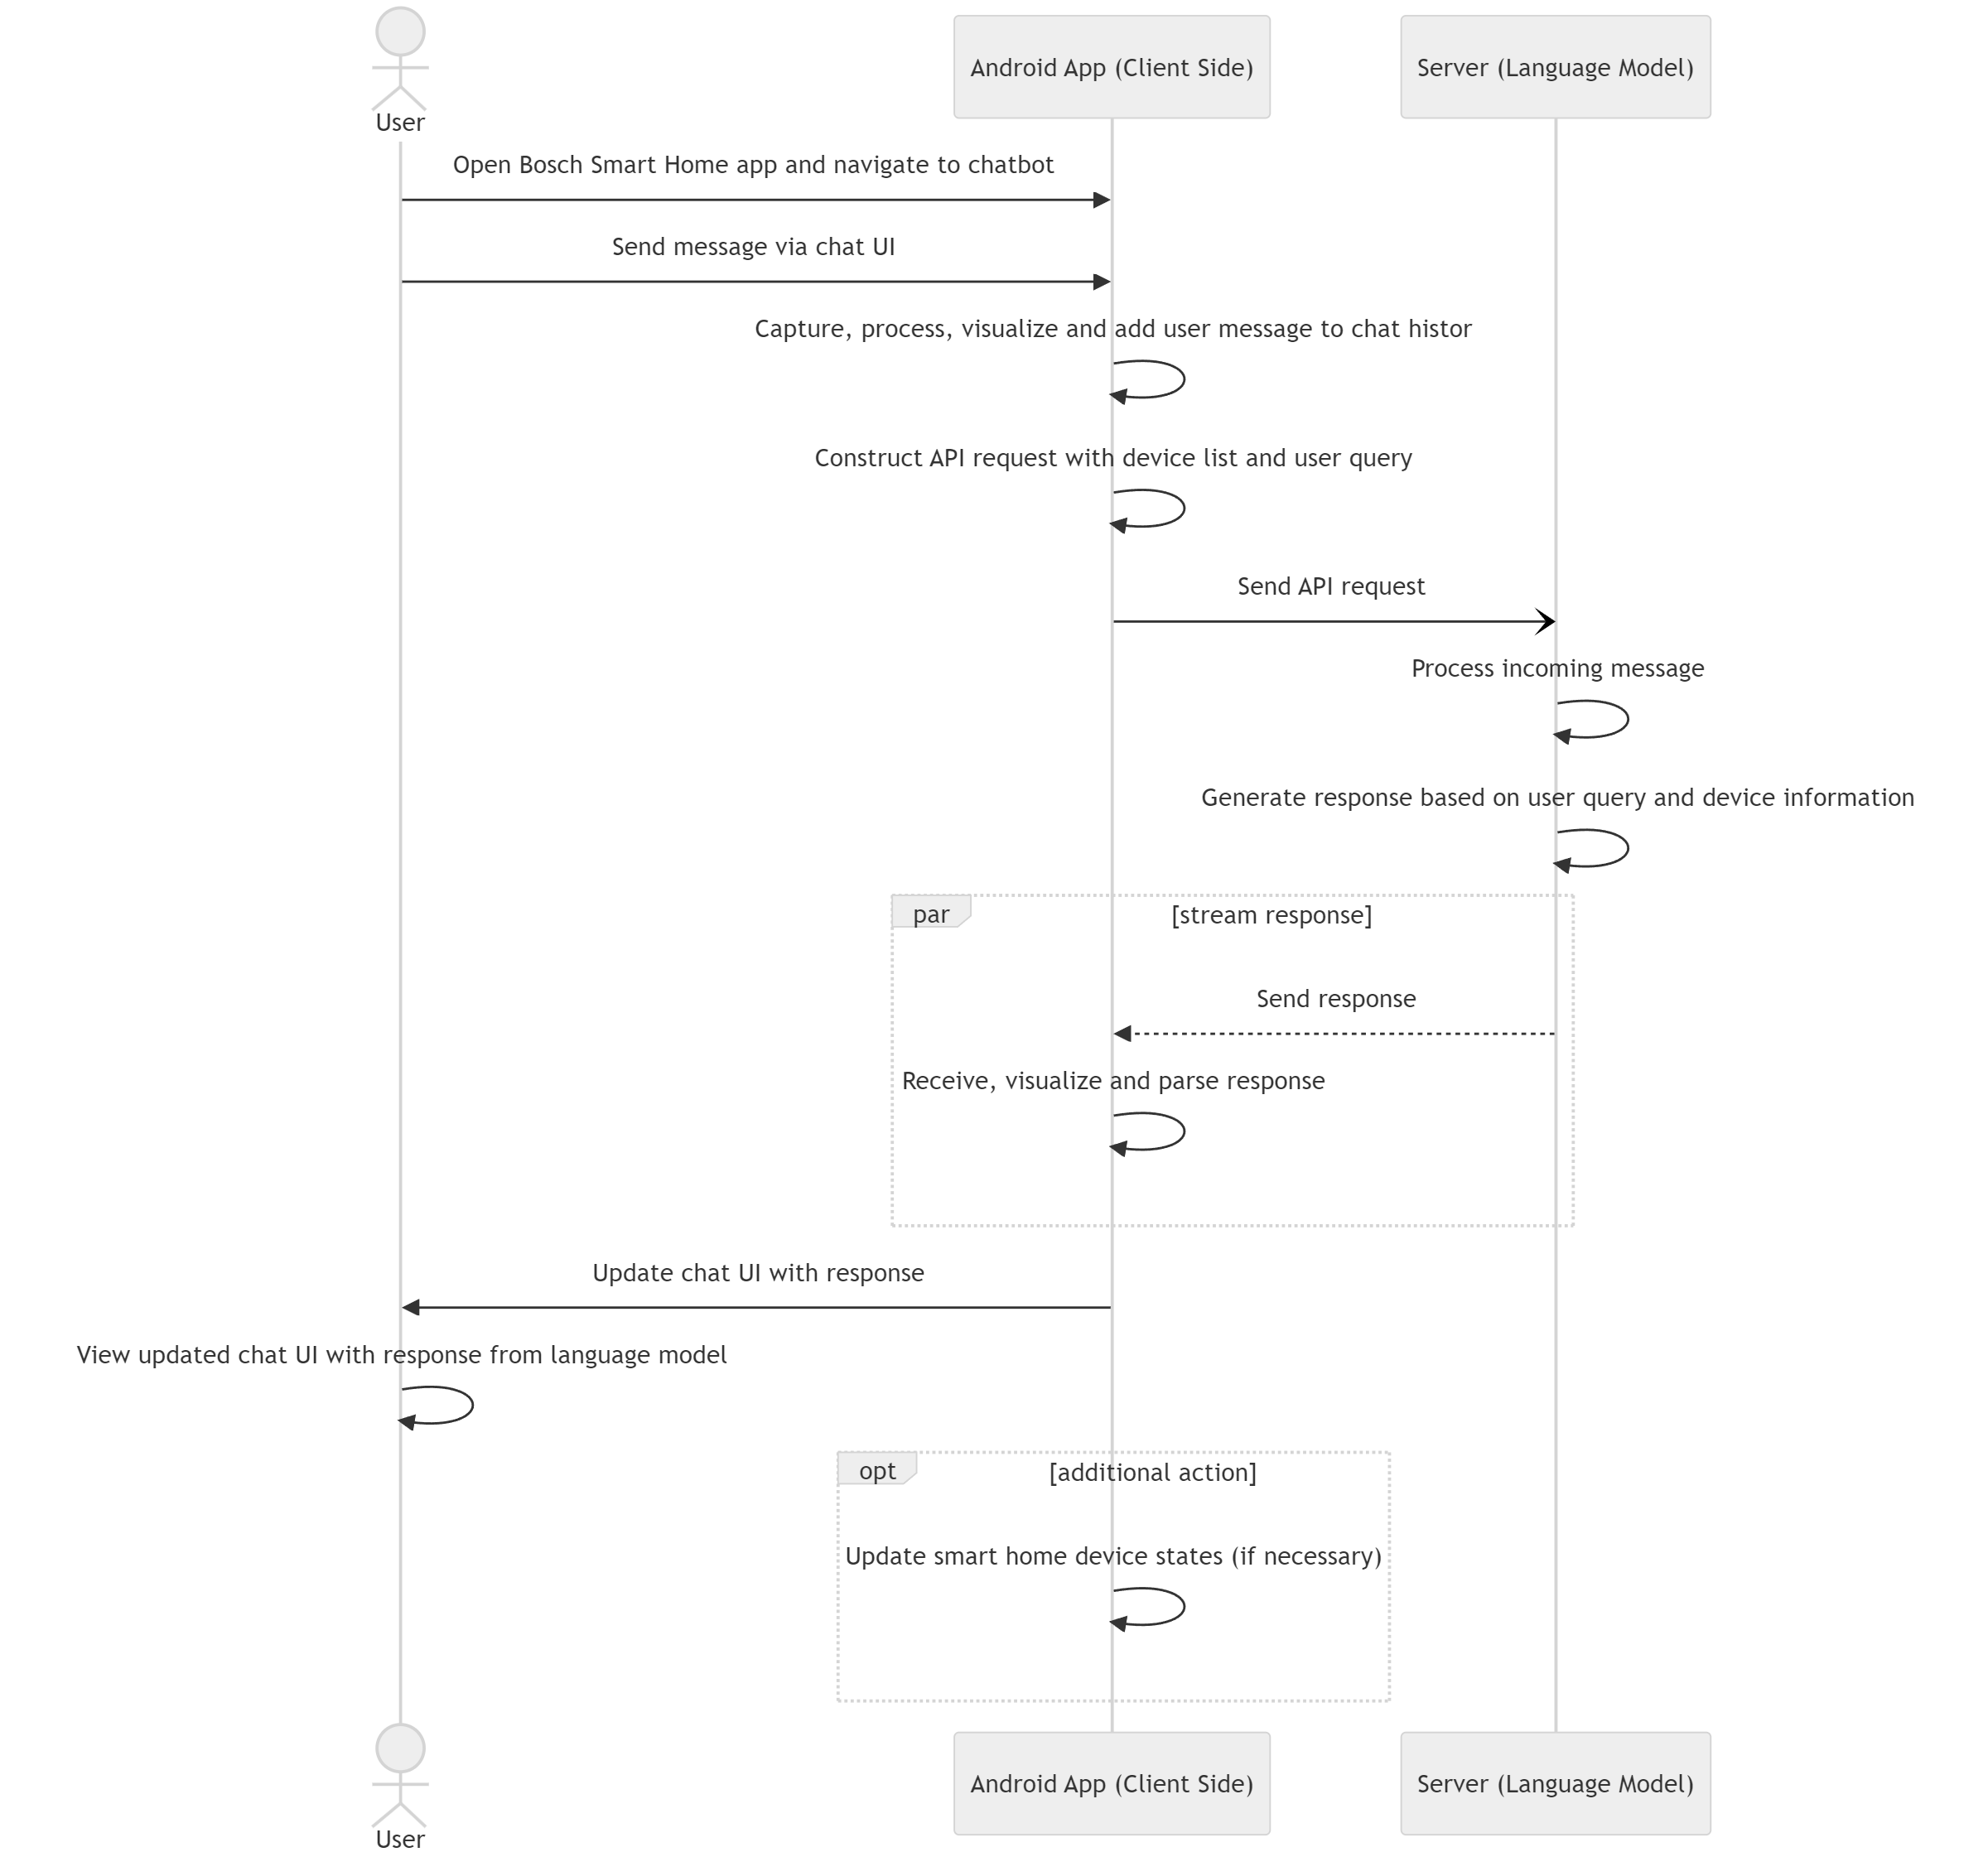
\includegraphics[width=\textwidth]{graphics/sequencedia.png}
    \caption{Sequence Diagram of the typical flow of the system}
    \label{fig:sequencedia}
\end{figure}
The interaction flow between the user, client-side application, and server is illustrated in Figure \ref{fig:sequencedia}. This sequence diagram outlines the process of handling user queries, constructing \gls{api} requests, and generating responses based on smart home device information.

The flow begins with user input via the chatbot interface. The client-side application then retrieves the current state of smart home devices and packages this information, along with the user's query and recent message history, into a structured \gls{api} request using the Request Builder module.
This request is sent to the server hosting the Ollama software and language model, which processes the input and generates a response. The response is streamed back to the client in real-time, enhancing user experience by reducing perceived latency.

The Response Handler module separates the incoming response into a natural language component and a structured \gls{json} object. The natural language portion is displayed in the \gls{ui}, while the \gls{json} object is parsed for any action directives.

If actions are specified, the Response Handler triggers the corresponding functions in the client application, potentially sending commands to smart home devices or updating the application's state. The \gls{ui} is then updated to reflect both the chatbot's response and any changes in device states.
This finishes the interaction loop. The entire process typically occurs within seconds.


\section{Challenges and Solutions}
\label{sec:challenges-solutions}
There were several challenges and considerations that had to be taken into account when designing and developing the prototype:

\textbf{Complexity of Automations}: Balancing simplicity and functionality in user-defined automations proved challenging. The vast possibilities of Bosch Smart Home automations made it difficult to build a comprehensive assistant. Even if the language model could understand the capabilities of the automations, mapping this to a \gls{json} output and triggering a function to create specific automations would be complex. A potential solution would have been to define a set of automation types that could be created, but time constraints prevented this development.
    
\textbf{Multilingual Support}: Providing accurate and contextually appropriate responses in both German and English was difficult in some scenarios. The chatbot occasionally struggled to consistently answer in German when the user's last input was in German, despite understanding the request. A possible reason could be that the device list provided to the model is always in English. Potential solutions include providing the model with information about the Bosch Smart Home app's current language, adapting the device list's language accordingly, or fine-tuning the model. Time limitations prevented the implementation of these solutions.

\textbf{Historical Data}: During the thesis, historical data of the Bosch Smart Home devices was not available. Only the current state of devices could be accessed. Some variables in this state store summarized historical data, such as the total power consumption for smart plugs. A potential solution could have been to mock the data to test what data format would be sufficient for the model to correctly answer user requests and interpret the data.

\textbf{Availability of System Logs}: Beginning with the second iteration of intents, system logs would have acted as a solid foundation for short-term historical data, including state changes of devices, automations, and errors. However, this information is only available inside the Bosch Smart Home Controller and therefore encapsulated from the Android App. Time constraints prevented the development of functionality to share these logs with the app.

\textbf{Data from External Sources}: Integrating data from external sources, such as the ``Statistisches Bundesamt'' (Federal Statistical Office of Germany), could have provided valuable insights for energy cost analysis in the user's home. This data, including information on inflation in energy costs (gas, district heating, electricity, etc.), could have been used to analyze why energy costs increased and offer suggestions for energy savings based on unnecessary automations. Implementing this would require data retrieval and ingestion from defined sources (URLs), potentially using \gls{rag} with Ollama or Langchain. While time constraints prevented the implementation of this feature in our prototype, we explored the necessary data and methods. Our experiments showed that providing the language model with a list of devices containing (artificial) historical data, information on related automations, and inflation indices gave sufficient context for reasoning, although not always with perfect accuracy.
    
\textbf{Security Issue}: The Bosch Smart Home app initially did not support \gls{api} calls to arbitrary domains. To address this, we needed to modify the security settings for the prototype to enable calls to the Ollama \gls{api} on a specific device. This change was implemented only for the chatbot functionality, while the rest of the app maintained its original security configuration.

\textbf{Model Performance}: Incrementally improving model outputs proved challenging. In our case, this was achieved by analyzing the output of our evaluation script, identifying low-quality outputs, and addressing them in the modelfile by adding more examples or instructive text. The evaluation script itself is described in \cref{sec:modelperform}.
%\blinddocument
